\documentclass[a4paper,12pt]{article}
\usepackage{graphicx} %Inserimento immagini
\usepackage{biblatex}
\usepackage{xcolor}
\newcommand\todo[1]{\textcolor{red}{\textbf{//TODO: \textit{#1}}}}


\title{Relazione progetto Ingegneria del Software}
\date{\parbox{\linewidth}{\centering
		\today\endgraf\bigskip
		Giosuè Corbioli (VR518264)\\
		Giovanni Grigoli (VR500669) \\
		Rey Merzari (VR517101) \\
		Denis Modenese (VR518328)\endgraf\bigskip
		Dip. Informatica\bigskip \endgraf
		Università degli studi di Verona}}


\renewcommand{\contentsname}{Contenuti}

\begin{document}
	
	\maketitle
	\newpage
	\tableofcontents
	\newpage
	\section{Introduzione}

Questo documento illustra la progettazione e lo sviluppo di un sistema informatico di telemedicina dedicato alla gestione clinica dei pazienti affetti da diabete di tipo 2.\\
L'architettura del sistema si basa sull'interazione tra due attori principali: \\
I pazienti utilizzano la piattaforma per registrare autonomamente le misurazioni glicemiche giornaliere, documentare l'assunzione di farmaci e segnalare eventuali sintomi, comorbidità e terapie concomitanti.\\
Il medico diabetologo può, tramite la piattaforma, assegnare piani terapeutici ai suoi pazienti, oltre che compilare e consultare la loro cartella clinica e visualizzare l'andamento della glicemia.\\
Il sistema prevede una funzionalità di autenticazione centralizzata gestita dai responsabili del servizio.\\

Nelle successive sezioni sono presentati i diagrammi UML utilizzati per la progettazione e modellazione dei requisiti, seguiti da un'analisi delle decisioni strutturali e architetturali prese.
 
 \clearpage
	\newpage
	\begin{landscape}
	\section{Class Diagram}
	
	\begin{figure}[H]
		\centering
		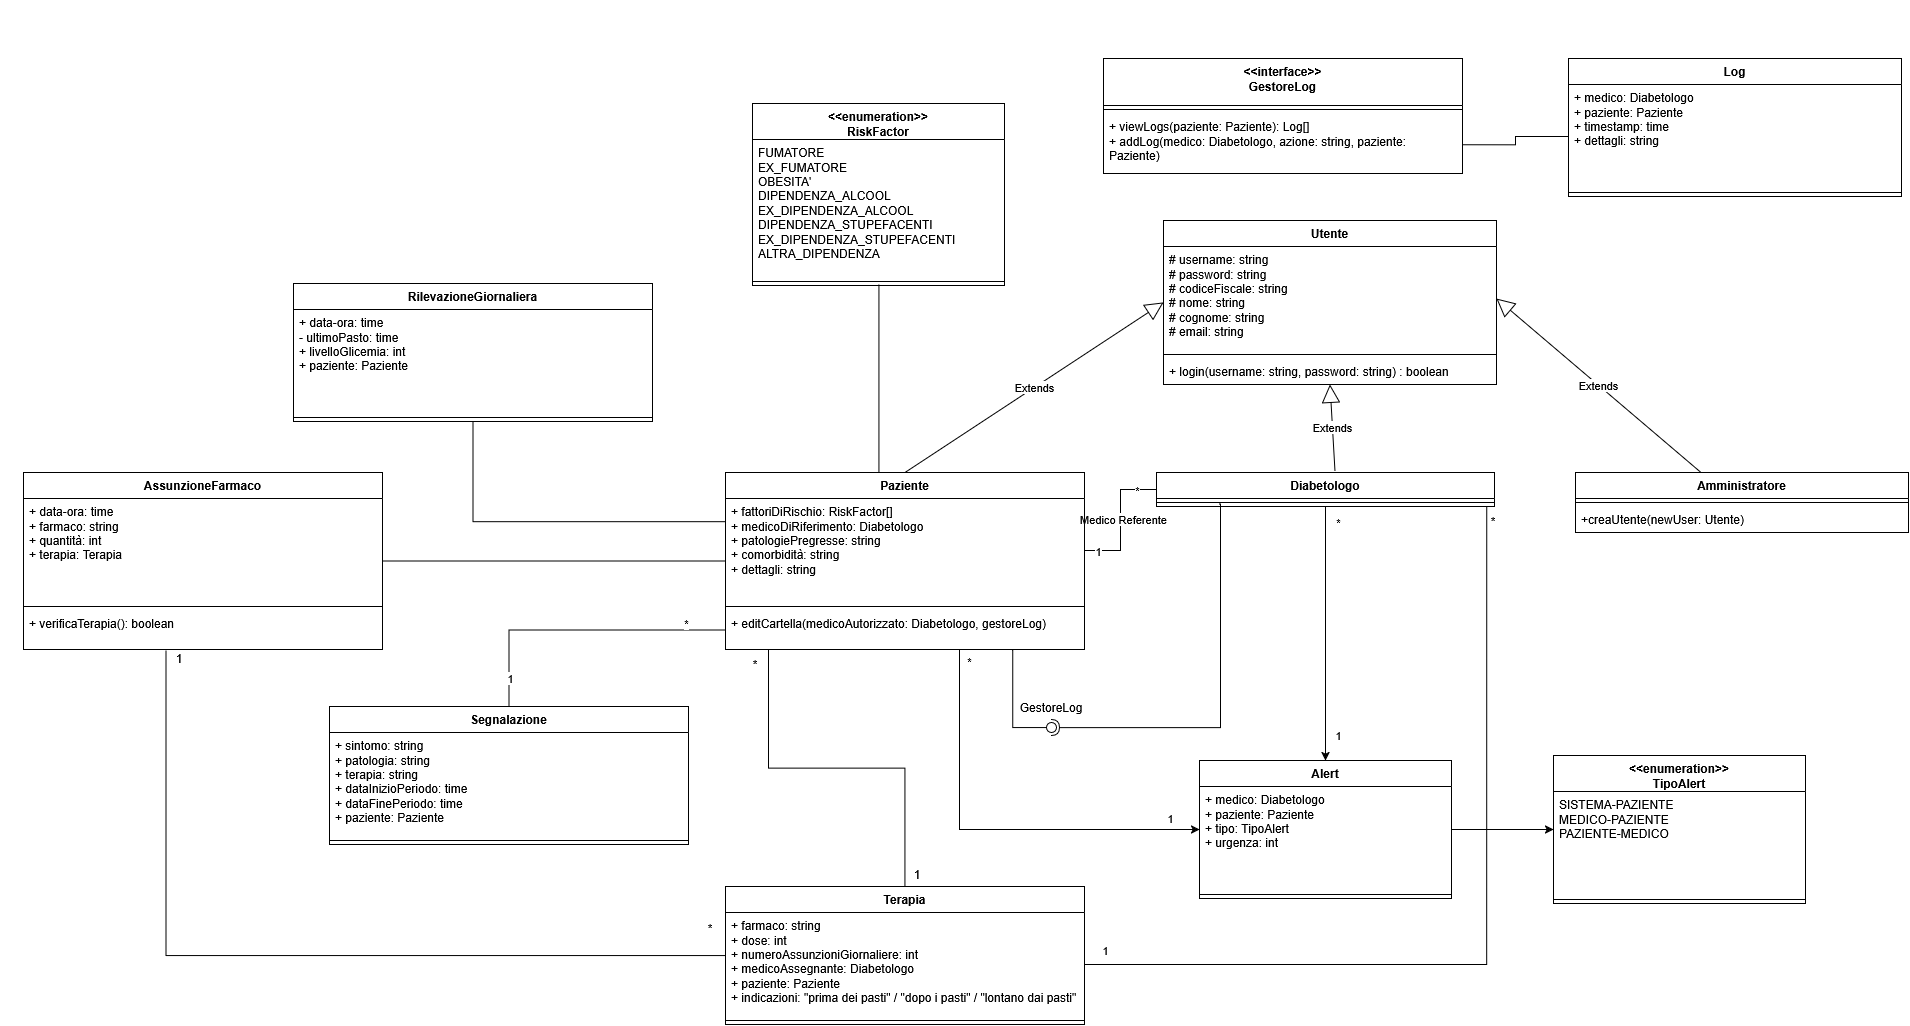
\includegraphics[
		width=1\linewidth,
		height=0.99\textheight,
		keepaspectratio
		]{Immagini/Bozza-UML(6).drawio.png}
		\caption{Class Diagram}
		\label{fig:class-diagram}
	\end{figure}
\end{landscape}

\clearpage

\subsection{Class Diagram della modellazione concettuale}

Il sistema è incentrato sulla classe astratta Utente, raccoglie i dati comuni ai diversi tipi di utilizzatori, quali username, password, codice fiscale, nome, cognome ed email. Da essa derivano le classi Paziente, Diabetologo e Responsabile.\\

A ogni Paziente è associato un Diabetologo come medico di riferimento. Il Paziente mantiene inoltre i propri fattori di rischio, rappresentati tramite  l'enumerazione RiskFactor, oltre che le proprie patologie pregresse, comorbidità e altri dettagli clinici. La modifica della cartella clinica (editCartella()) richiede l'autorizzazione di un medico e viene registrata tramite l'interfaccia GestoreLog, che salva ogni operazione in un oggetto Log (medico, paziente, timestamp, dettagli), in modo da assicurare il requisito di tracciabilità delle operazioni dei medici.\\
Le rilevazioni giornaliere registrano data e ora, ultimo pasto e livello di glicemia. Le assunzioni di farmaci sono verificate rispetto alla Terapia assegnata tramite verificaTerapia().\\
Il paziente può inoltre effettuare Segnalazioni relative a sintomi, patologie o altre situazioni rilevanti. Il sistema gestisce messaggi tra paziente e diabetologo e genera messaggi di sistema destinati al paziente o al medico in presenza di condizioni che richiedono attenzione, come valori glicemici fuori soglia o mancata aderenza alla terapia.\\

Il Diabetologo può visualizzare i pazienti di propria competenza, consultare il loro andamento glicemico e gestire le relative terapie e informazioni cliniche.
La classe Terapia contiene le informazioni relative al farmaco prescritto, alla dose, al numero di assunzioni giornaliere, al medico assegnante e alle indicazioni. Una stessa terapia può essere associata a più pazienti. Quando una terapia condivisa viene modificata per un singolo paziente, viene creata una nuova terapia per evitare di modificare quella degli altri pazienti.\\

Il Responsabile è incaricato della gestione degli utenti del sistema, in particolare della creazione e modifica dei dati relativi a pazienti e diabetologi.\\

La persistenza dei dati è garantita dalla classe Database, che centralizza il caricamento, il salvataggio, l'inserimento, la modifica e il recupero delle informazioni memorizzate nel file del database.

\begin{landscape}
	\section{Class Diagram del software}
	
	\begin{figure}[H]
		\centering
		\includesvg[
		width=0.99\linewidth,
		height=0.99\textheight,
		keepaspectratio
		]{Immagini/UmlSpecifico}
		\caption{Class Diagram del software}
		\label{fig:class-diagram-software}
	\end{figure}
\end{landscape}

\clearpage

 \textcolor{red}{TODO: METTERE}

	\newpage
	\section{Use Case Diagram}

 \begin{figure}[H]
	\makebox[\paperwidth][c]{
		\hspace*{-7.5cm}
		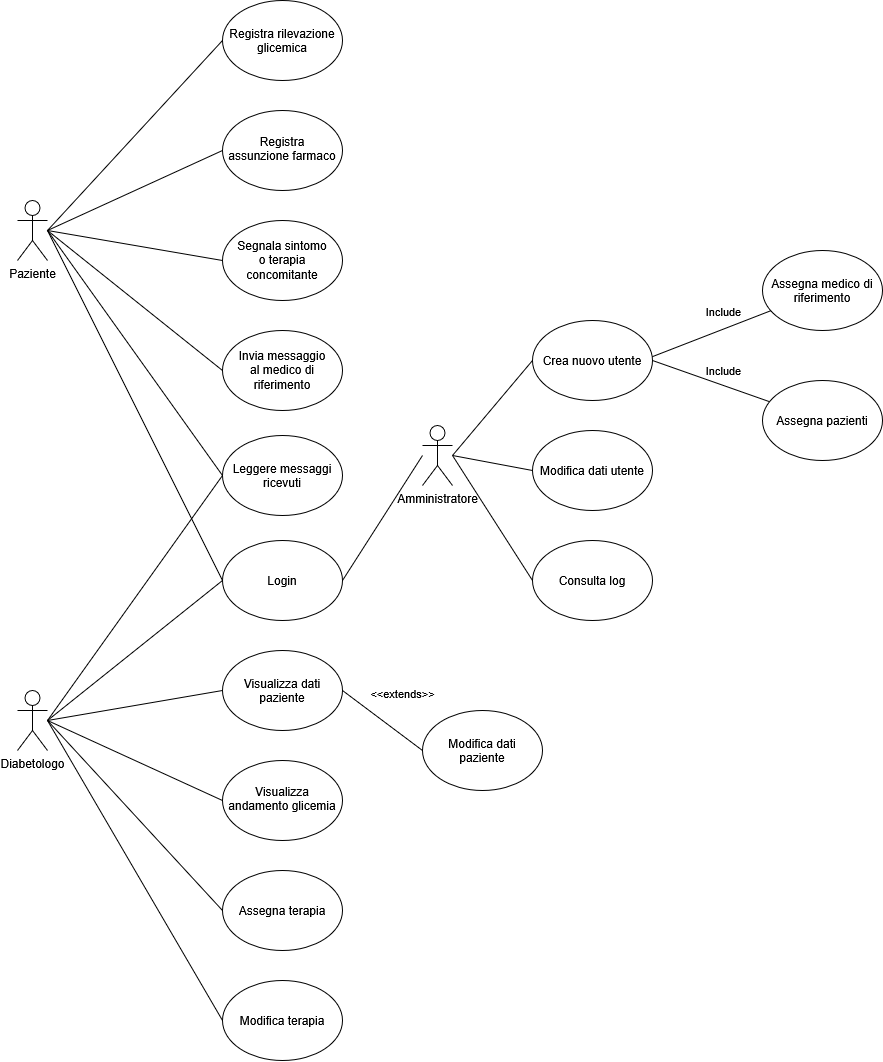
\includegraphics[
		height=0.94\textheight,
		keepaspectratio
		]{Immagini/UseCaseDiagram.png}
	}
	\label{fig:use-case-diagram}
\end{figure}

\clearpage

\begin{figure}[H]
	\centering
	
	\makebox[\paperwidth][c]{
		\hspace*{-7.5cm}
		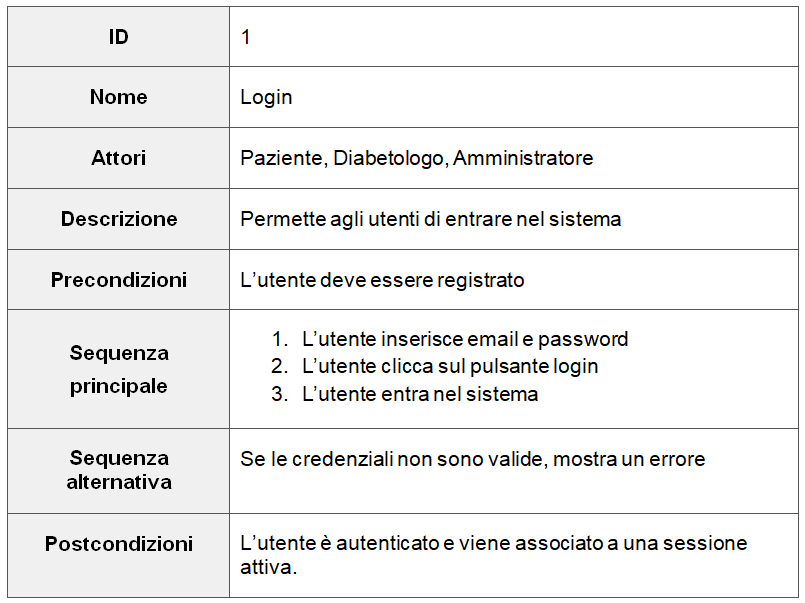
\includegraphics[
		height=0.49\textheight,
		keepaspectratio
		]{Immagini/UseCase1.png}
	}
	
	\vspace{0.1cm}
	
	\makebox[\paperwidth][c]{
		\hspace*{-7.5cm}
		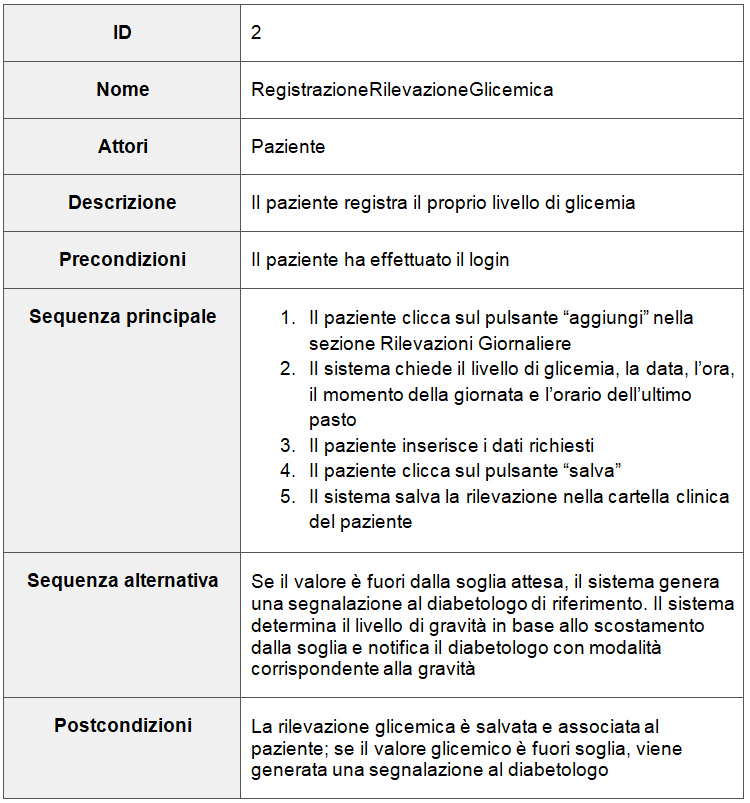
\includegraphics[
		height=0.50\textheight,
		keepaspectratio
		]{Immagini/UseCase2.png}
	}
	
	\label{fig:use-case-1-2}
\end{figure}

\begin{figure}[H]
	\centering
	
	\makebox[\paperwidth][c]{
		\hspace*{-7.5cm}
		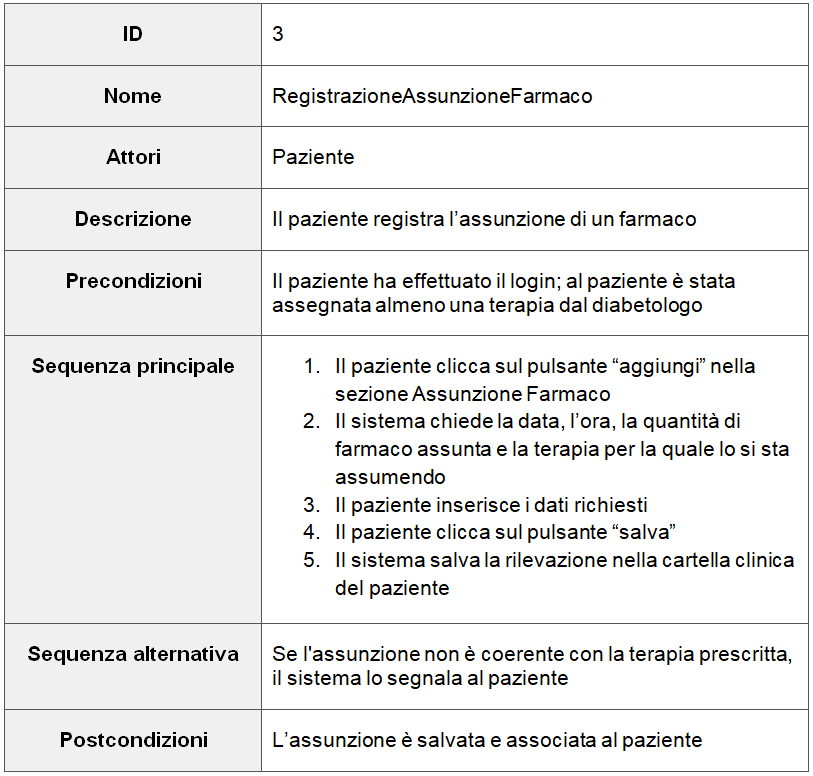
\includegraphics[
		height=0.49\textheight,
		keepaspectratio
		]{Immagini/UseCase3.png}
	}
	
	\vspace{0.1cm}
	
	\makebox[\paperwidth][c]{
		\hspace*{-7.5cm}
		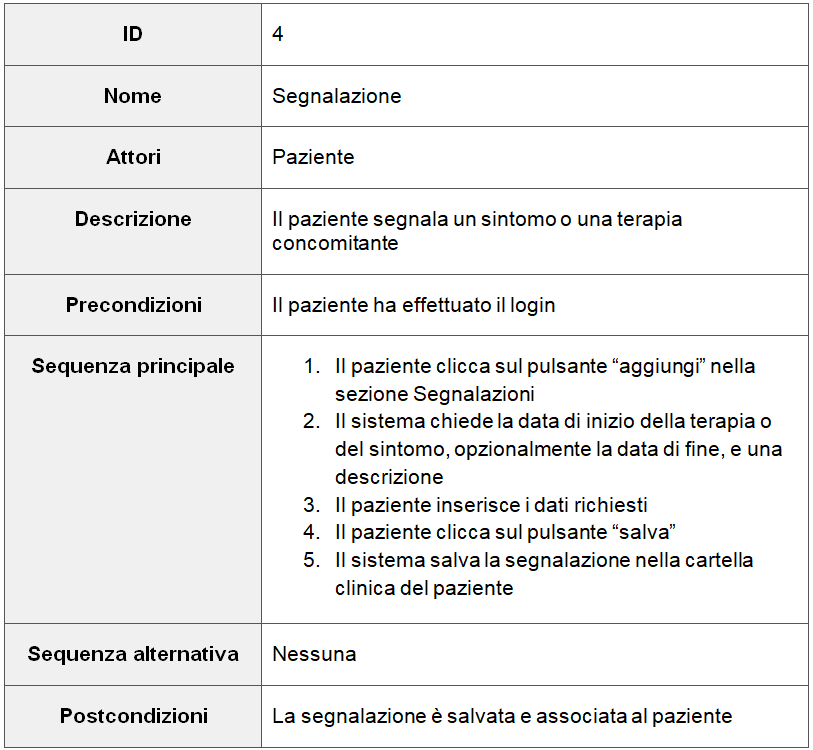
\includegraphics[
		height=0.50\textheight,
		keepaspectratio
		]{Immagini/UseCase4.png}
	}
	
	\label{fig:use-case-3-4}
\end{figure}


\begin{figure}[H]
	\centering
	
	\makebox[\paperwidth][c]{
		\hspace*{-7.5cm}
		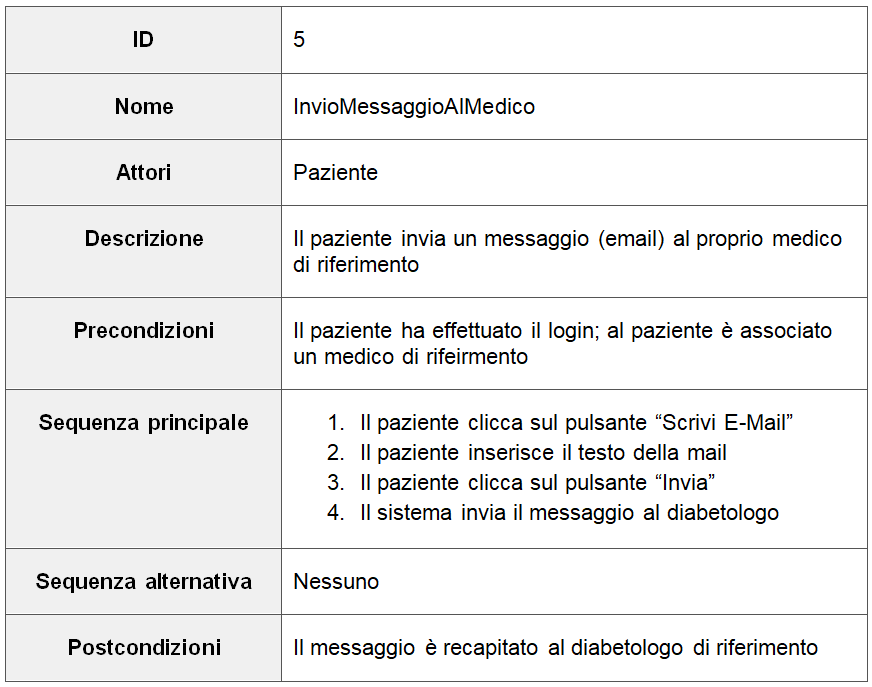
\includegraphics[
		height=0.49\textheight,
		keepaspectratio
		]{Immagini/UseCase5.png}
	}
	
	\vspace{0.1cm}
	
	\makebox[\paperwidth][c]{
		\hspace*{-7.5cm}
		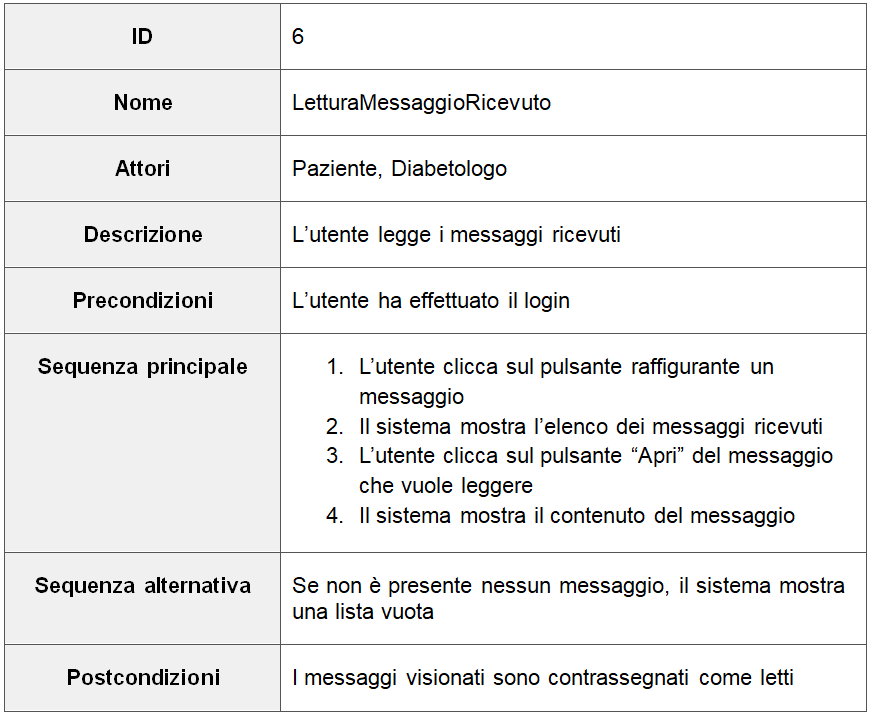
\includegraphics[
		height=0.50\textheight,
		keepaspectratio
		]{Immagini/UseCase6.png}
	}
	
	\label{fig:use-case-5-6}
\end{figure}


\begin{figure}[H]
	\centering
	
	\makebox[\paperwidth][c]{
		\hspace*{-7.5cm}
		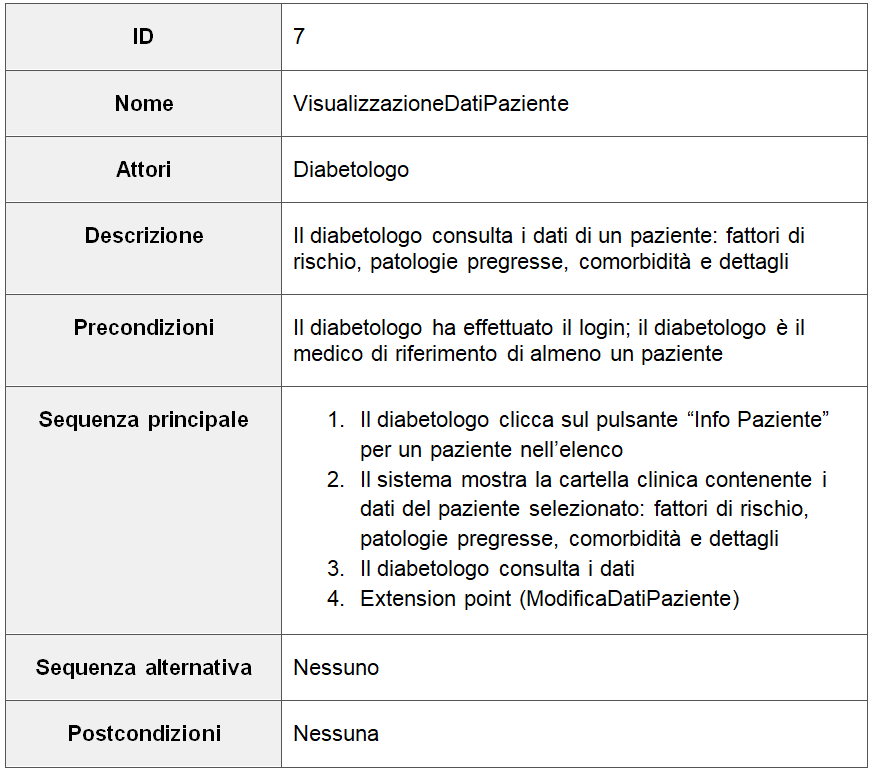
\includegraphics[
		height=0.49\textheight,
		keepaspectratio
		]{Immagini/UseCase7.png}
	}
	
	\vspace{0.1cm}
	
	\makebox[\paperwidth][c]{
		\hspace*{-7.5cm}
		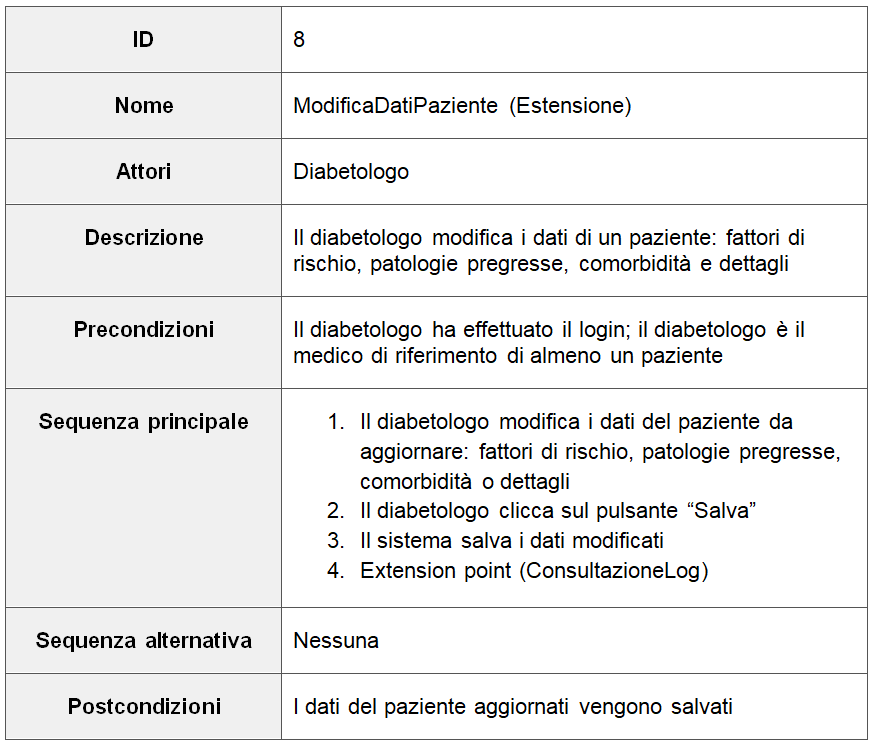
\includegraphics[
		height=0.50\textheight,
		keepaspectratio
		]{Immagini/UseCase8.png}
	}
	
	\label{fig:use-case-7-8}
\end{figure}


\begin{figure}[H]
	\centering
	
	\makebox[\paperwidth][c]{
		\hspace*{-7.5cm}
		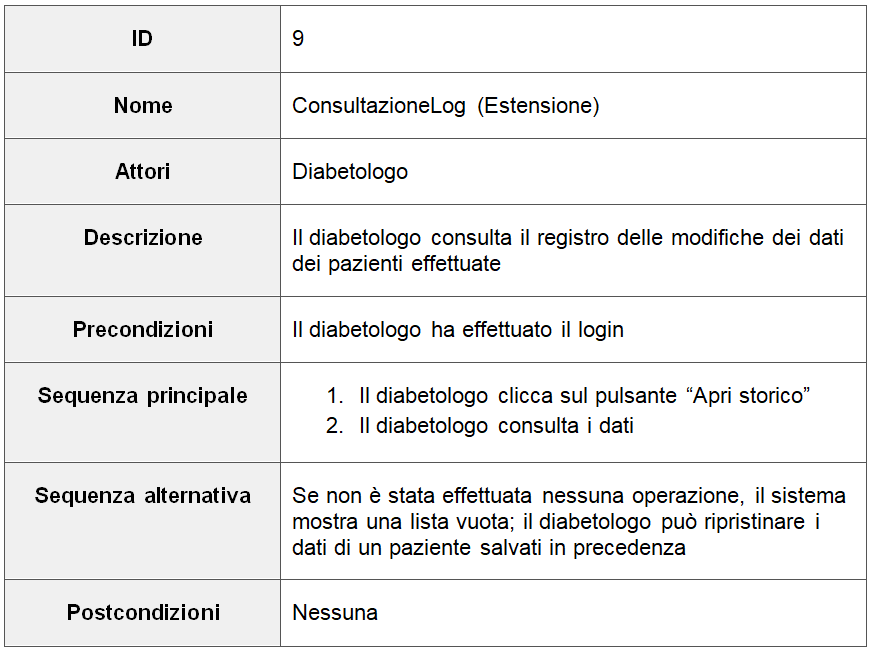
\includegraphics[
		height=0.49\textheight,
		keepaspectratio
		]{Immagini/UseCase9.png}
	}
	
	\vspace{0.1cm}
	
	\makebox[\paperwidth][c]{
		\hspace*{-7.5cm}
		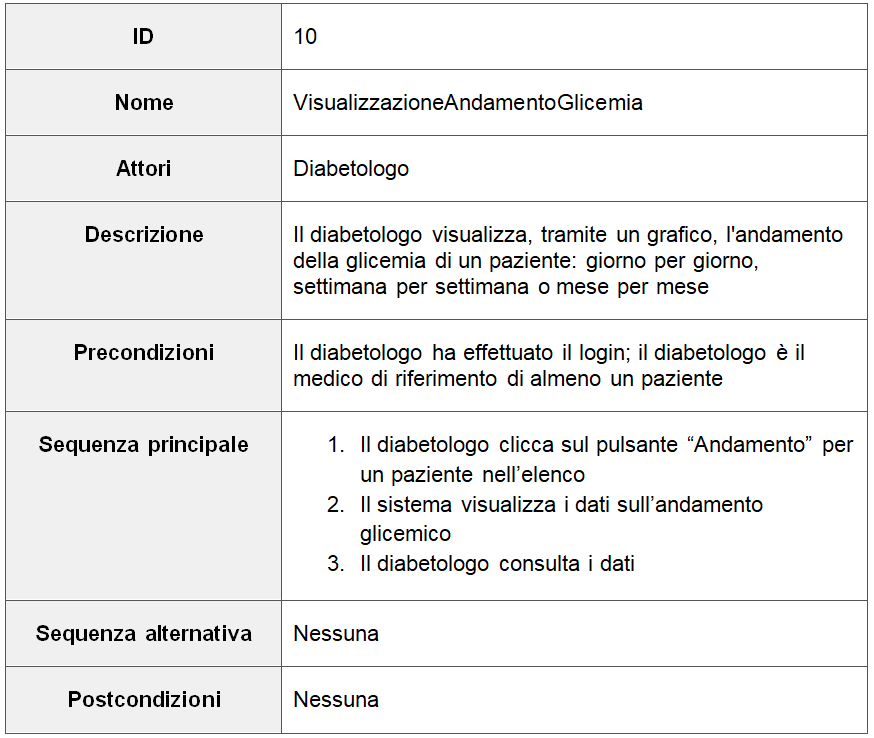
\includegraphics[
		height=0.50\textheight,
		keepaspectratio
		]{Immagini/UseCase10.png}
	}
	
	\label{fig:use-case-9-10}
\end{figure}


\begin{figure}[H]
	\centering
	
	\makebox[\paperwidth][c]{
		\hspace*{-7.5cm}
		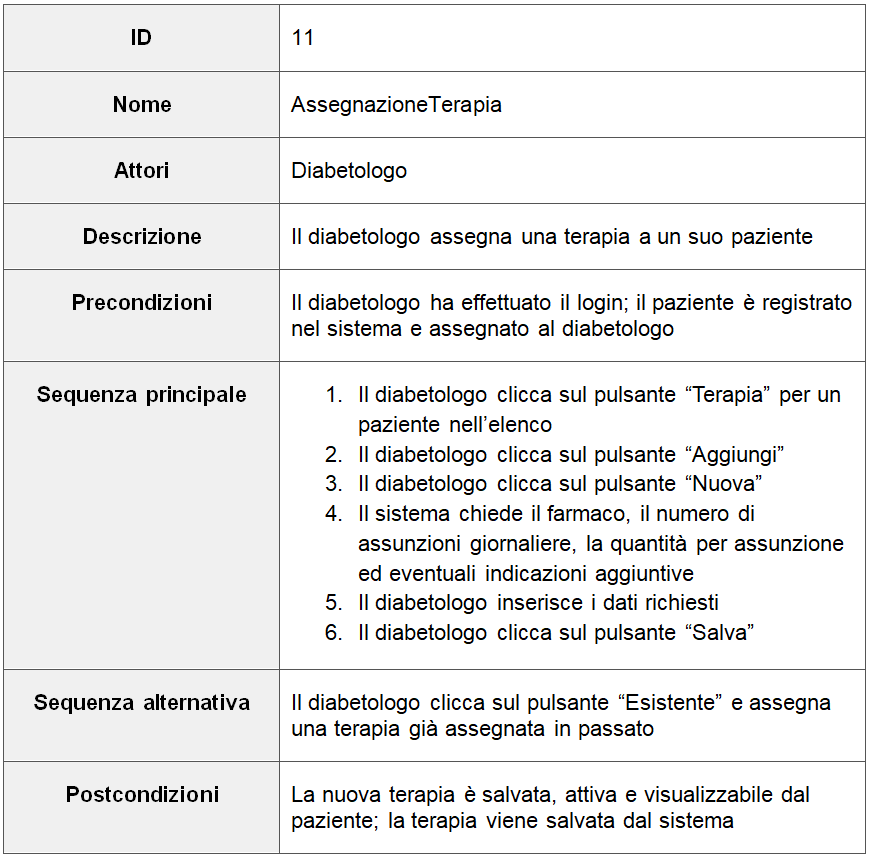
\includegraphics[
		height=0.49\textheight,
		keepaspectratio
		]{Immagini/UseCase11.png}
	}
	
	\vspace{0.1cm}
	
	\makebox[\paperwidth][c]{
		\hspace*{-7.5cm}
		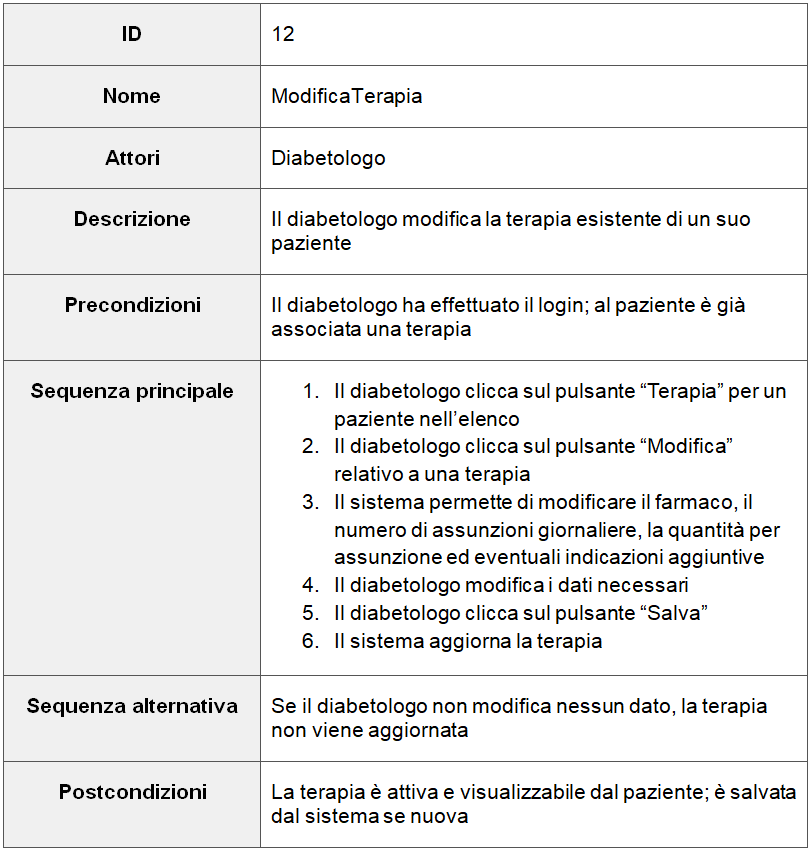
\includegraphics[
		height=0.50\textheight,
		keepaspectratio
		]{Immagini/UseCase12.png}
	}
	
	\label{fig:use-case-11-12}
\end{figure}


\begin{figure}[H]
	\centering
	
	\makebox[\paperwidth][c]{
		\hspace*{-7.5cm}
		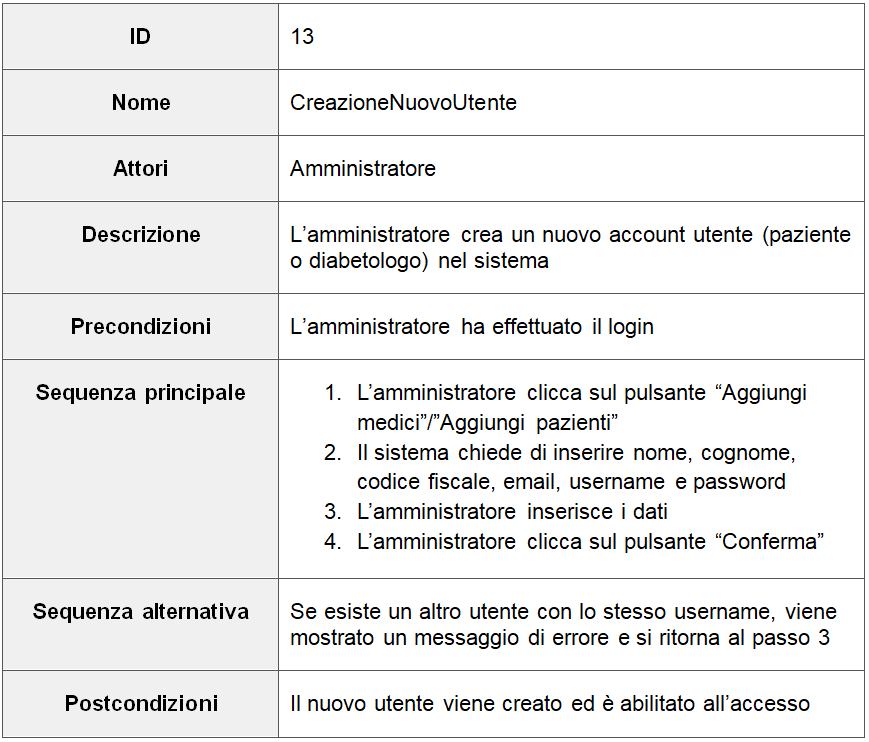
\includegraphics[
		height=0.49\textheight,
		keepaspectratio
		]{Immagini/UseCase13.png}
	}
	
	\vspace{0.1cm}
	
	\makebox[\paperwidth][c]{
		\hspace*{-7.5cm}
		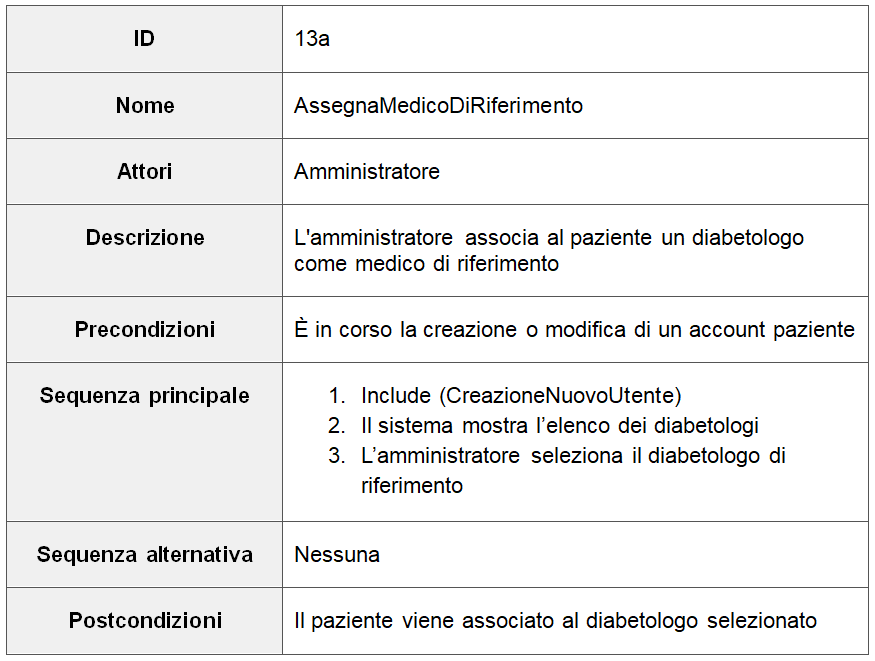
\includegraphics[
		height=0.50\textheight,
		keepaspectratio
		]{Immagini/UseCase13a.png}
	}
	
	\label{fig:use-case-13-13a}
\end{figure}


\begin{figure}[H]
	\centering
	
	\makebox[\paperwidth][c]{
		\hspace*{-7.5cm}
		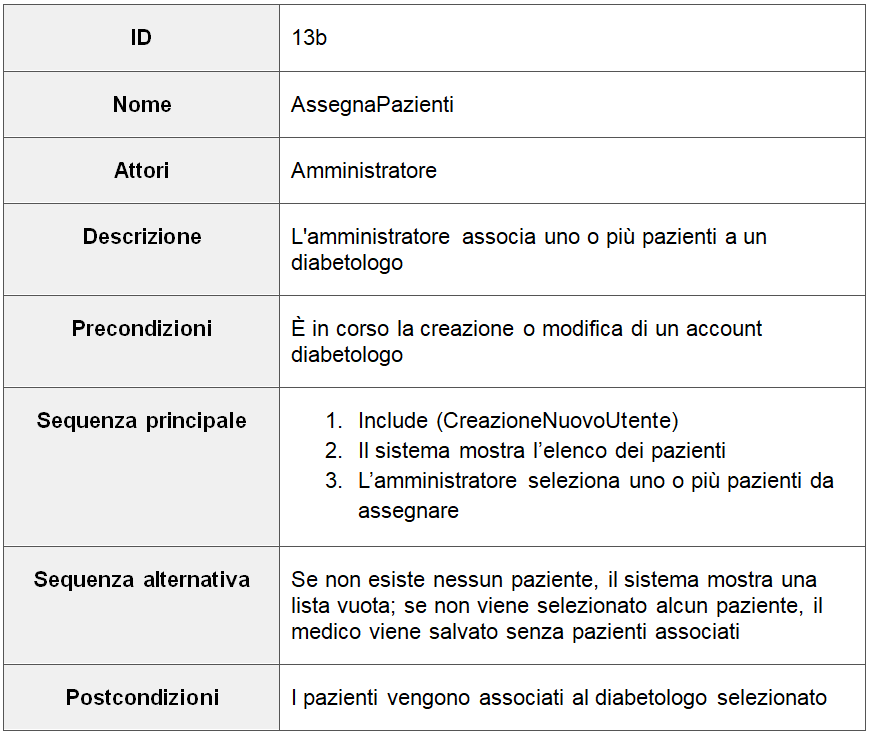
\includegraphics[
		height=0.49\textheight,
		keepaspectratio
		]{Immagini/UseCase13b.png}
	}
	
	\vspace{0.1cm}
	
	\makebox[\paperwidth][c]{
		\hspace*{-7.5cm}
		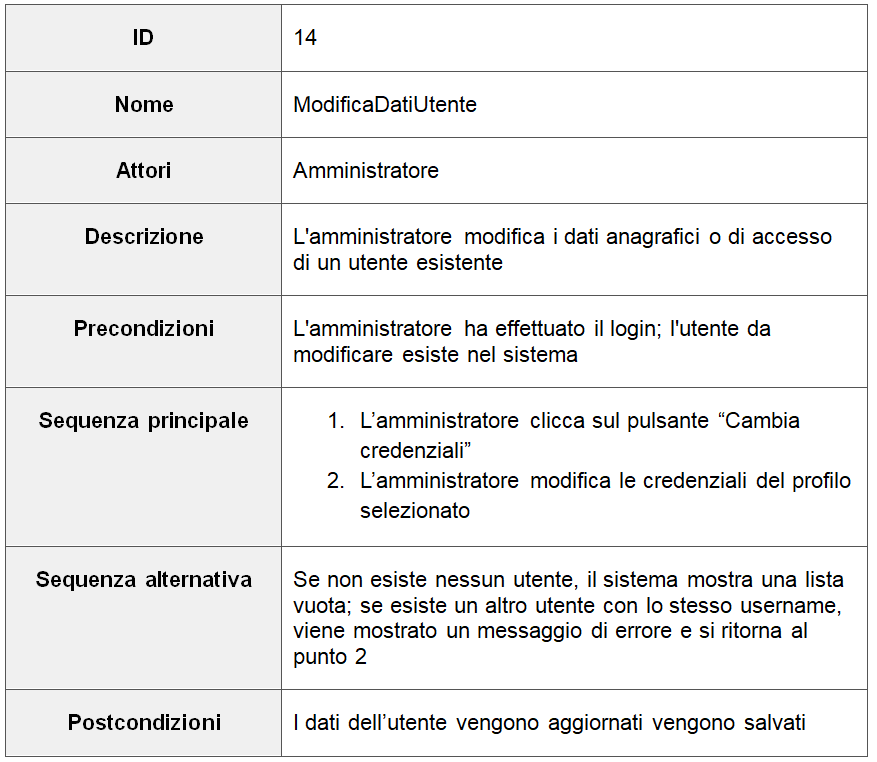
\includegraphics[
		height=0.50\textheight,
		keepaspectratio
		]{Immagini/UseCase14.png}
	}
	
	\label{fig:use-case-13b-14}
\end{figure}
 
	\newpage
	\section{Sequence Diagram}

\begin{figure}[H]
	\makebox[\paperwidth][c]{
		\hspace*{-7.5cm}
		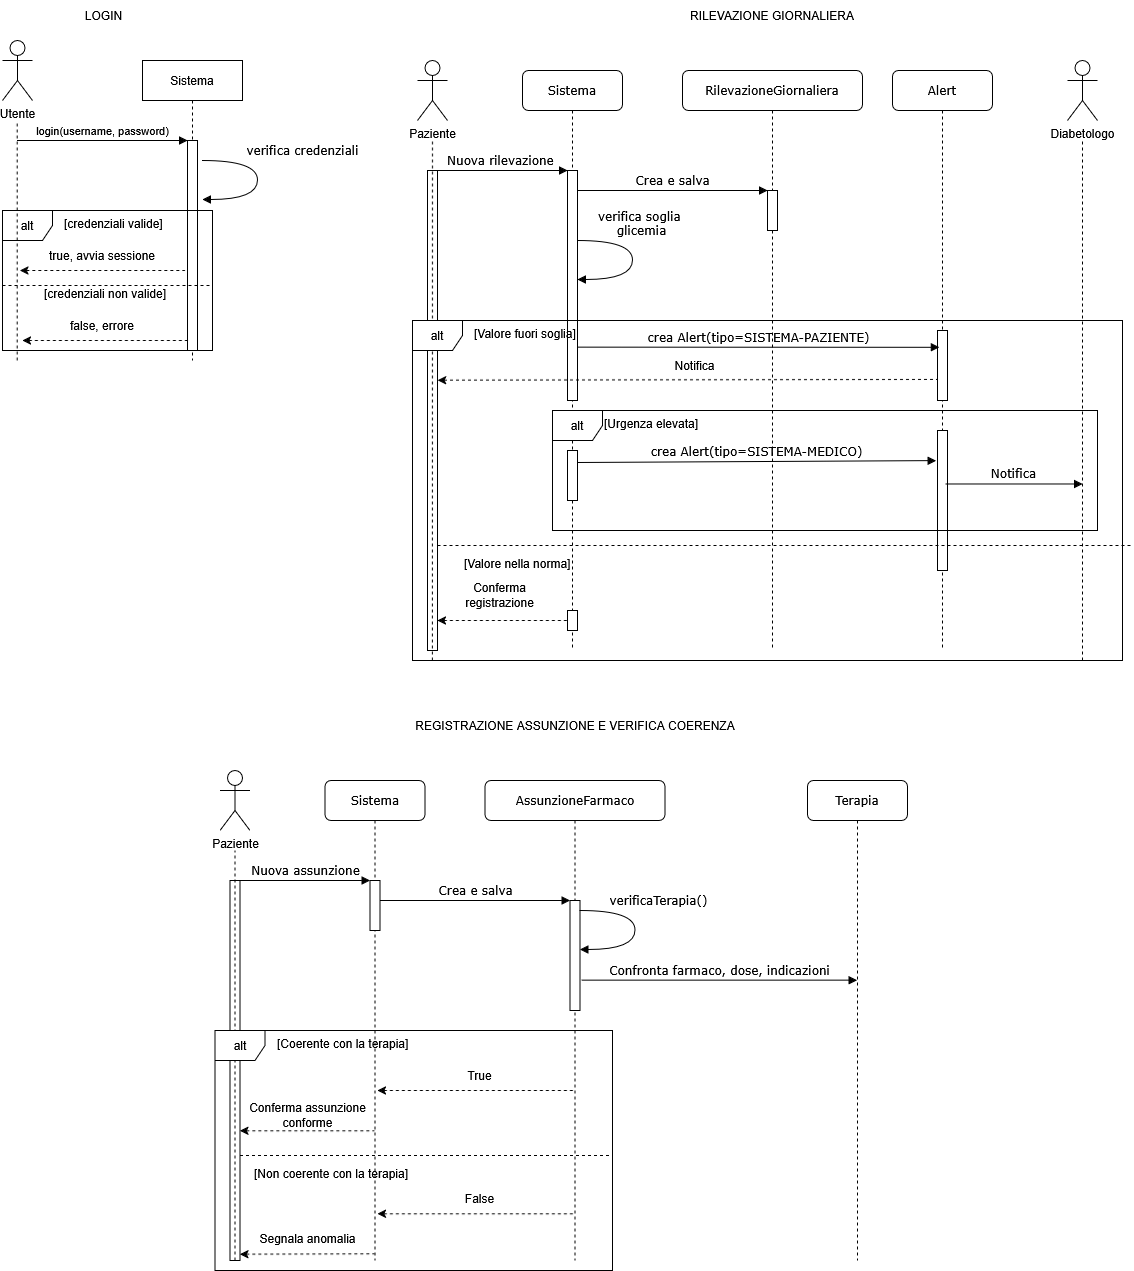
\includegraphics[
		height=0.92\textheight,
		keepaspectratio
		]{Immagini/SequenceDiagram11.png}
	}
	\caption{Sequence Diagram (Parte 1)}
	\label{fig:sequence-diagram_1}
\end{figure}

\begin{figure}[H]
	\makebox[\paperwidth][c]{
		\hspace*{-7.5cm}
		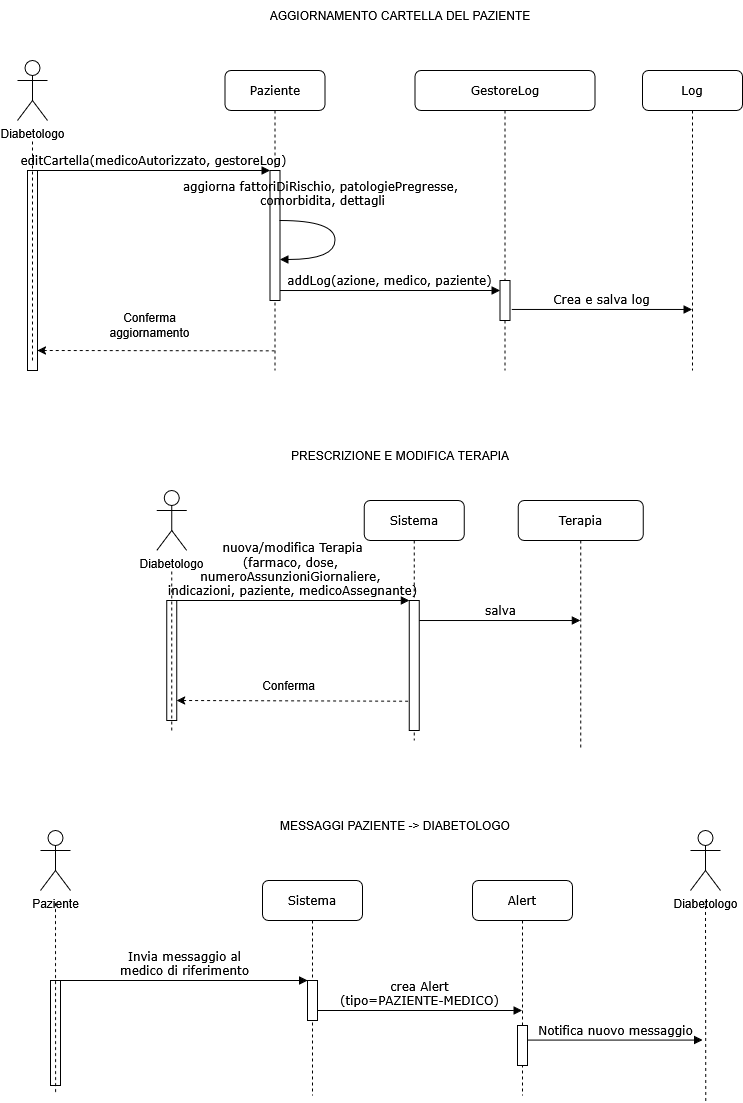
\includegraphics[
		width=0.98\paperwidth,
		height=0.98\textheight,
		keepaspectratio
		]{Immagini/SequenceDiagram33.png}
	}
	\caption{Sequence Diagram (Parte 2)}
	\label{fig:sequence-diagram_2}
\end{figure}

Login: L'utente inserisce username e password nella schermata di accesso. Il sistema inoltra le credenziali al database, il quale verifica la corrispondenza con un utente registrato. Se sono valide, viene avviata la sessione ed è aperta la schermata corrispondente al ruolo dell'utente. In caso contrario il sistema segnala un errore e  impedisce l'accesso.\\

Rilevazione giornaliera: il paziente inserisce i dati relativi a una nuova rilevazione, ovvero data, livello di glicemia, orario, orario dell'ultimo pasto e momento della rilevazione. Dopodiché il sistema la salva e verifica il livello di glicemia riportato rispetto alle soglie previste. Se esso è fuori dai limiti, viene creato un alert che notifica il diabetologo di riferimento di tale irregolarità, con un livello di urgenza maggiore se la glicemia si discosta particolarmente dalla norma. Il sistema conferma infine l'avvenuta  registrazione all'utente.\\

Registrazione di un'assunzione e verifica della coerenza: il paziente inserisce i dati relativi all'assunzione di un farmaco, indicando data, orario, quantità e terapia di riferimento. Tali dati vengono salvati e verificati, confrontandoli con le informazioni della terapia prescritta dal medico. Se essi sono discrepanti con la terapia, ciò viene segnalato all'utente.

Aggiornamento cartella del paziente: il diabetologo di riferimento accede alle informazioni del paziente e ne  modifica i dati, ovvero fattori di rischio, patologie pregresse, comorbidità e dettagli aggiuntivi. I dati vengono salvati e viene creato un log dell'operazione, associando la modifica all'utente che l'ha effettuata, in modo da mantenere la tracciabilità delle modifiche apportate.\\ 

Prescrizione e modifica di una terapia: il diabetologo di riferimento crea una nuova terapia oppure modifica le specifiche di una terapia già assegnata in passato modificando i dati rilevanti. Nel caso di modifica di una terapia condivisa da più pazienti, il sistema crea una nuova versione della terapia per il paziente interessato, evitando di modificare la terapia degli altri pazienti che continuano a utilizzare quella precedente.\\

Scambio di messaggi tra paziente e diabetologo: il paziente apre la schermata di comunicazione e scrive un messaggio al proprio medico di riferimento. Il medico viene notificato, può aprirlo e leggerlo.
 
 \section{Sequence Diagram del software progettato}
 
 \begin{figure}[H]
 	\centering
 	
 	\makebox[\paperwidth][c]{
 		\hspace*{-7.5cm}
 		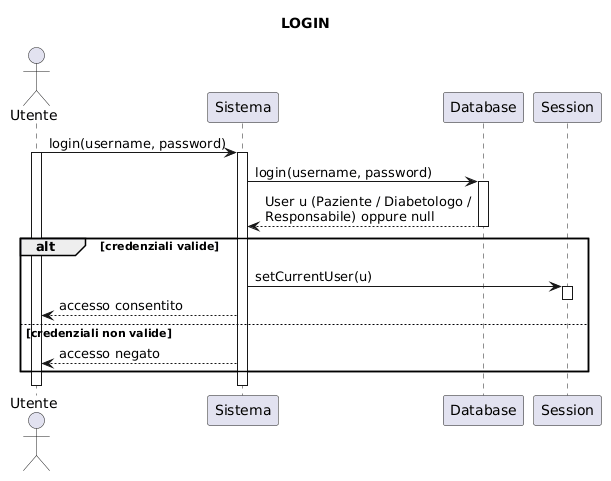
\includegraphics[
 		height=0.4\textheight,
 		keepaspectratio
 		]{Immagini/SequenceDiagramSW1.png}
 	}
 	
 	\vspace{0.1cm}
 	
 	\makebox[\paperwidth][c]{
 		\hspace*{-7.5cm}
 		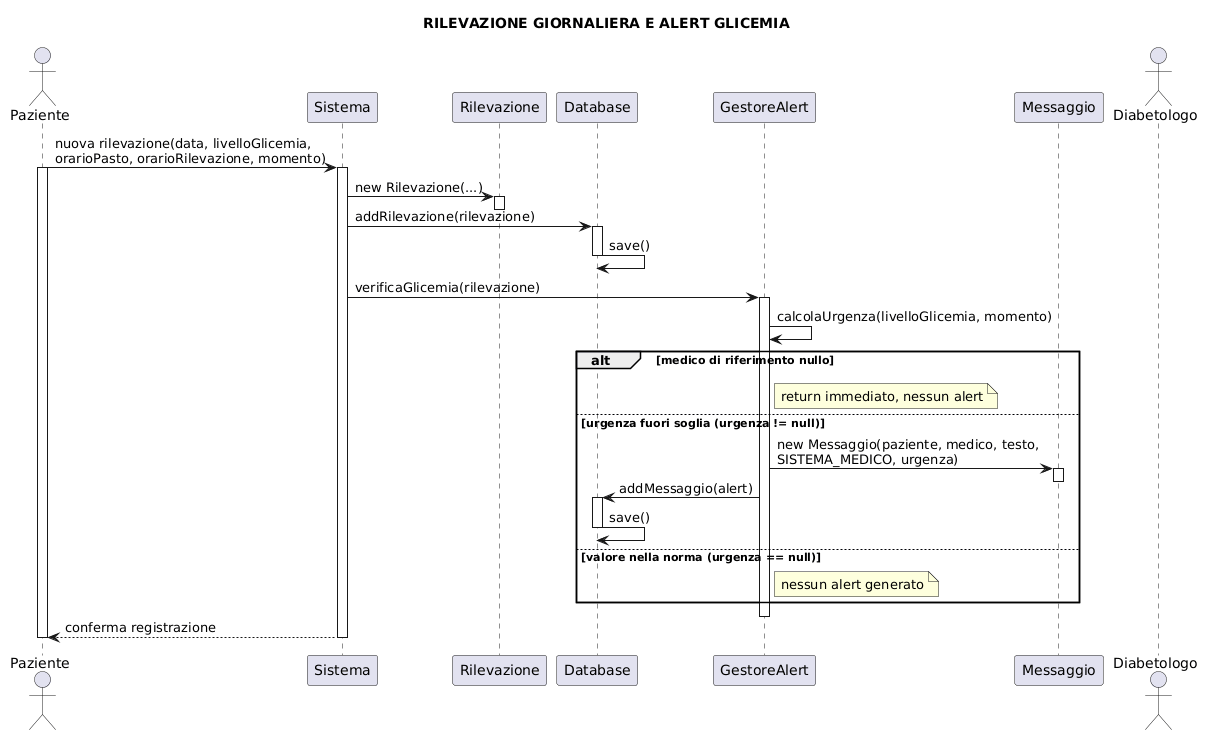
\includegraphics[
 		height=0.59\textheight,
 		keepaspectratio
 		]{Immagini/SequenceDiagramSW2.png}
 	}
 	
 	\label{fig:SD SF 1-2}
 \end{figure}
 
  \begin{figure}[H]
 	\centering
 	
 	\makebox[\paperwidth][c]{
 		\hspace*{-7.5cm}
 		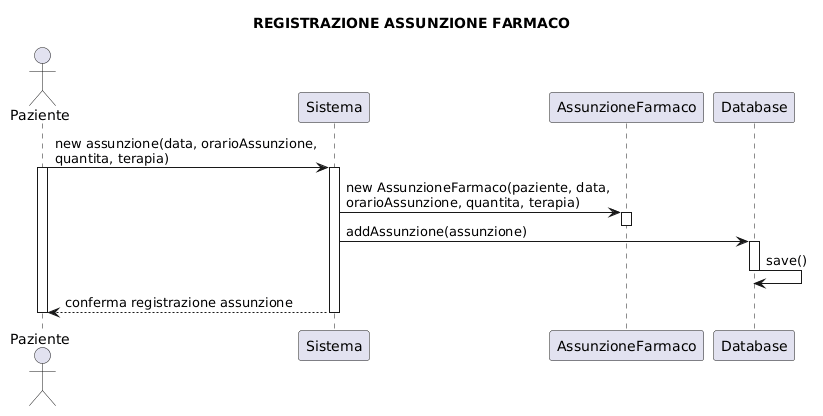
\includegraphics[
 		height=0.35\textheight,
 		keepaspectratio
 		]{Immagini/SequenceDiagramSW3.png}
 	}
 	
 	\vspace{0.1cm}
 	
 	\makebox[\paperwidth][c]{
 		\hspace*{-7.5cm}
 		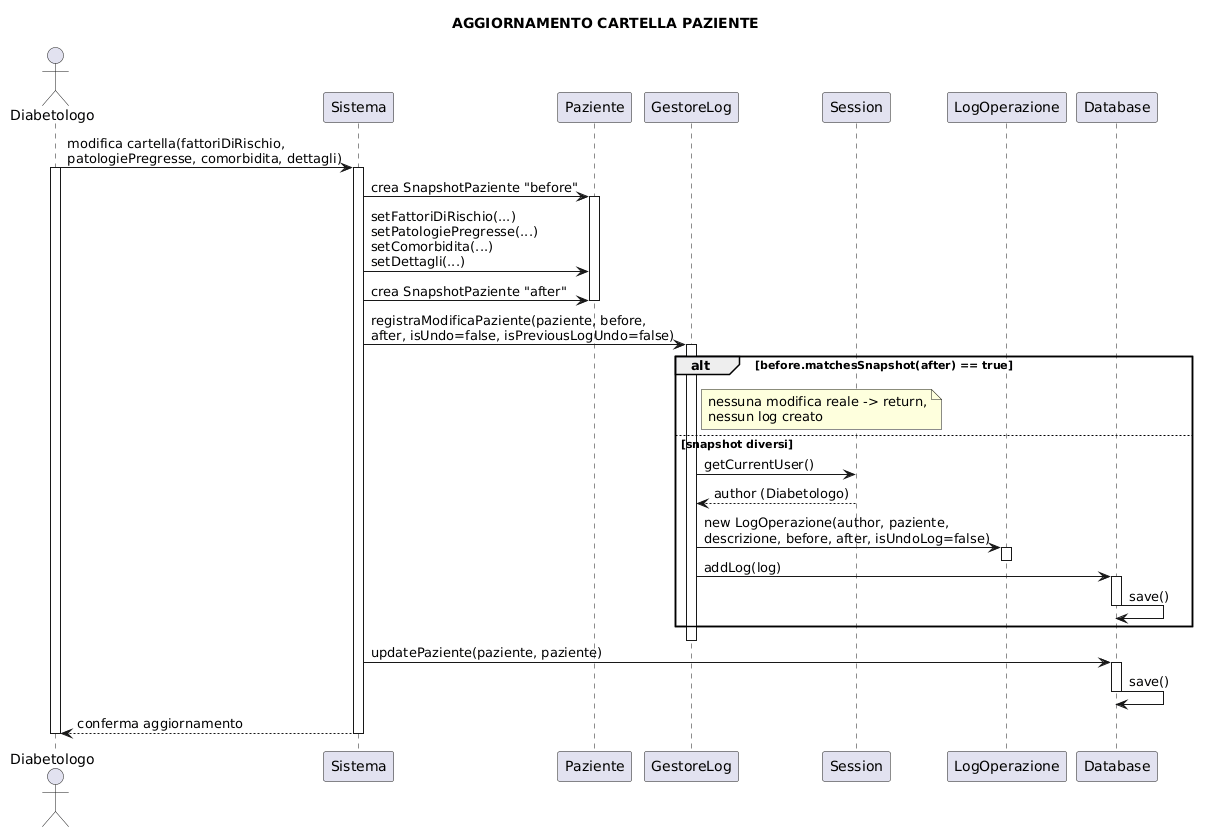
\includegraphics[
 		height=0.64\textheight,
 		keepaspectratio
 		]{Immagini/SequenceDiagramSW5.png}
 	}
 	
 	\label{fig:SD SF 3-5}
 \end{figure}
 
   \begin{figure}[H]
 	\centering
 	
 	\makebox[\paperwidth][c]{
 		\hspace*{-7.5cm}
 		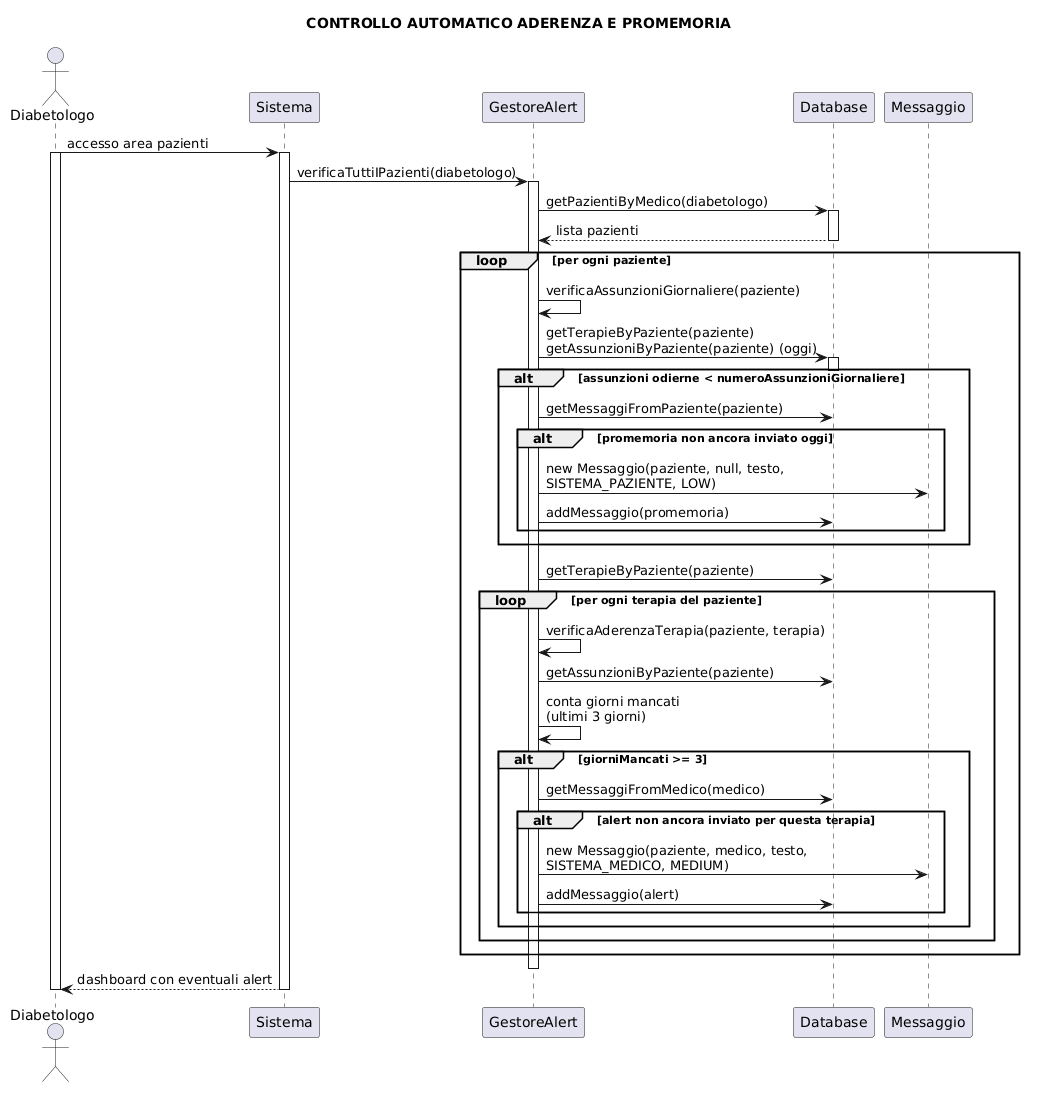
\includegraphics[
 		height=0.99\textheight,
 		keepaspectratio
 		]{Immagini/SequenceDiagramSW4.png}
 	}
 	 \label{fig:SD SF 4}

 \end{figure}
 
   \begin{figure}[H]
 	\centering
 	
 	\makebox[\paperwidth][c]{
 		\hspace*{-7.5cm}
 		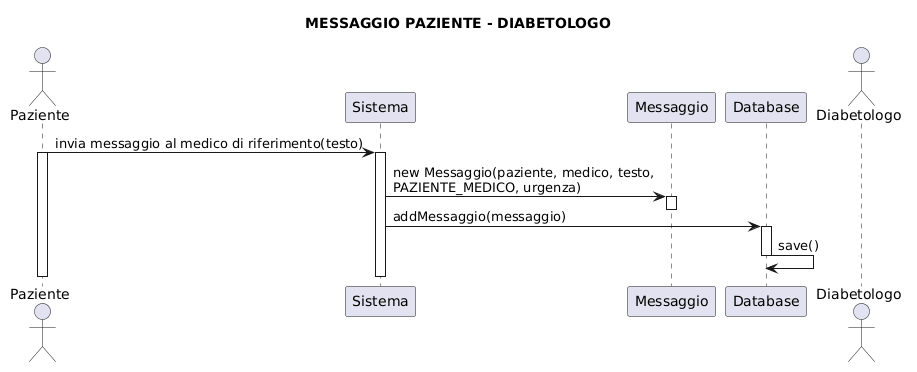
\includegraphics[
 		height=0.35\textheight,
 		keepaspectratio
 		]{Immagini/SequenceDiagramSW6.png}
 	}
 	
 	\vspace{0.1cm}
 	
 \makebox[\paperwidth][c]{
 	\hspace*{-7.5cm}
 	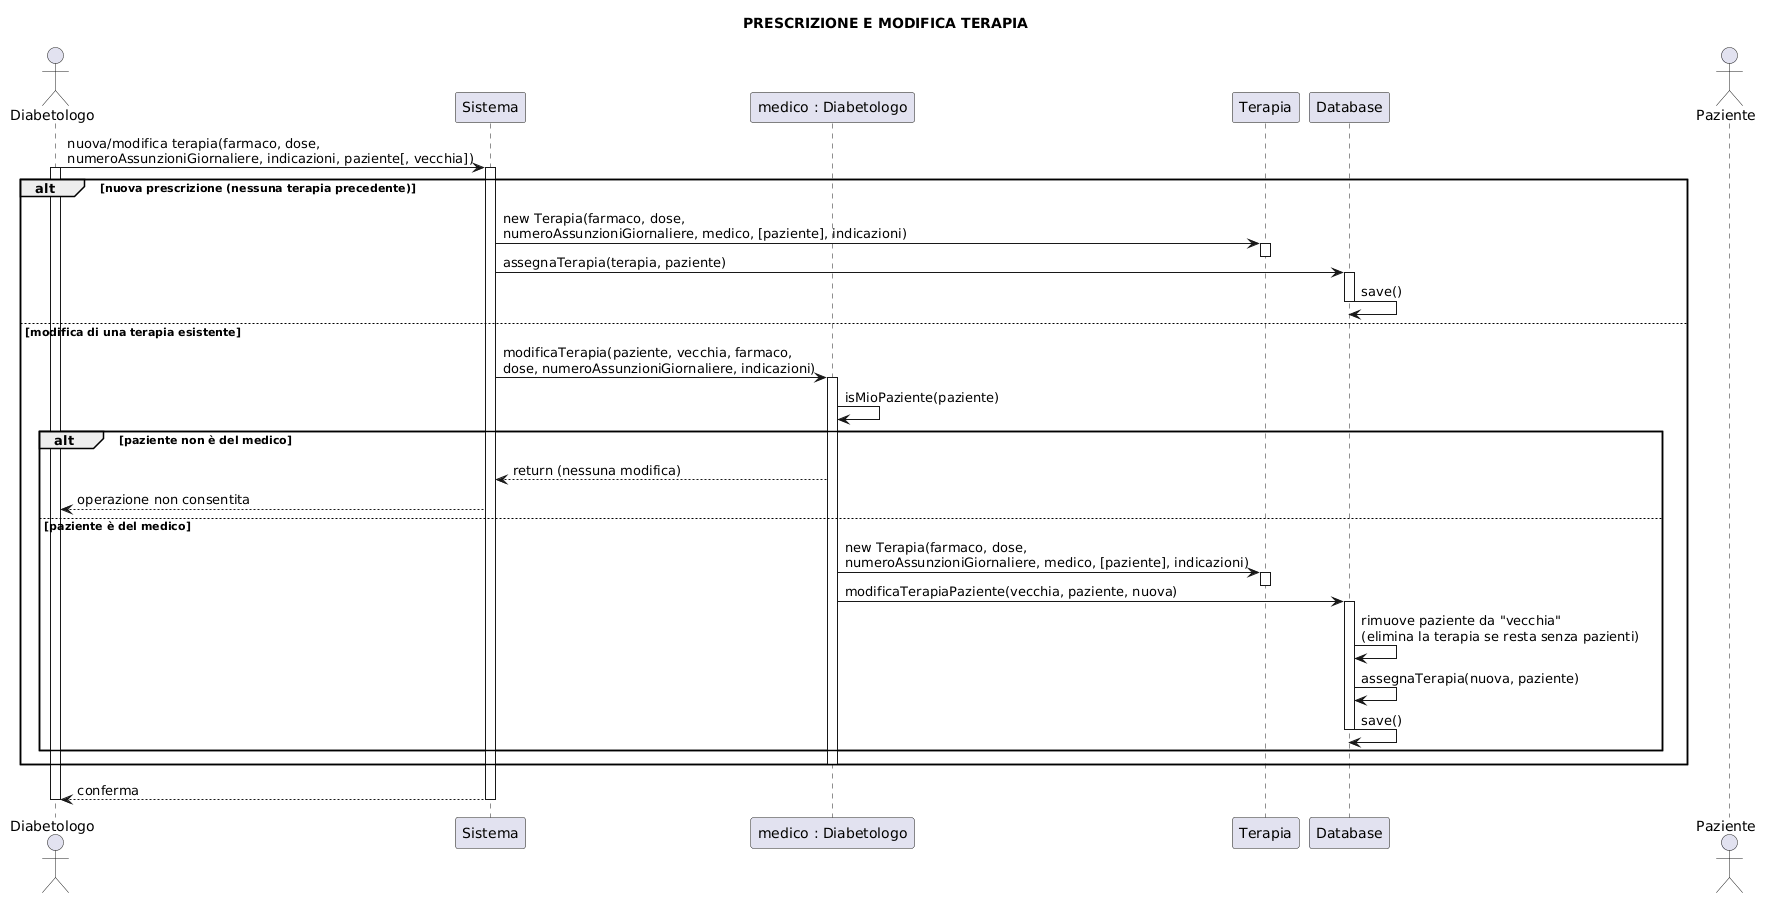
\includegraphics[
 	width=20cm,
 	height=0.7\textheight
 	]{Immagini/SequenceDiagramSW7.png}
 }
 	
 	\label{fig:SD SF 6-7}
 \end{figure}
 
Login: l'utente inserisce username e password nella schermata di accesso. Il sistema inoltra le credenziali al database, il quale verifica la corrispondenza con un utente registrato (Paziente, Diabetologo o Responsabile) oppure restituisce un valore nullo nel caso le credenziali non siano valide. Se sono valide, il sistema registra l'utente come corrente nella sessione attiva e consente l'accesso; in caso contrario, l'accesso viene negato.\\

Rilevazione giornaliera e alert glicemia: il paziente inserisce i dati di una nuova rilevazione (data, livello di glicemia, orario dell'ultimo pasto, orario della rilevazione e momento della giornata). Il sistema crea la rilevazione e la salva nel database, poi ne verifica il livello di glicemia rispetto alle soglie previste. Se il paziente non ha un medico di riferimento assegnato, il controllo termina senza generare alcun alert. Se invece il valore risulta fuori soglia, viene creato un messaggio di allerta destinato al medico, con un grado di urgenza calcolato in base a quanto il valore si discosta dalla norma, e il messaggio viene salvato nel database. Se il valore è nella norma, non viene generato alcun alert. In ogni caso, il sistema conferma al paziente l'avvenuta registrazione della rilevazione.\\

Registrazione assunzione farmaco: il paziente comunica al sistema l'avvenuta assunzione di un farmaco, specificando data, orario, quantità e terapia di riferimento. Il sistema crea l'oggetto assunzione e lo salva nel database, quindi conferma al paziente la registrazione avvenuta.\\

Controllo automatico aderenza e promemoria: quando il diabetologo accede all'area dei propri pazienti, il sistema avvia una verifica automatica su tutti i pazienti a lui assegnati. Per ciascun paziente, controlla innanzitutto se le assunzioni di farmaco registrate nella giornata sono inferiori al numero previsto dalla terapia: in tal caso, se non è già stato inviato un promemoria nella stessa giornata, ne viene generato uno a bassa urgenza destinato al paziente. Successivamente, per ogni terapia assegnata al paziente, il sistema conta i giorni mancati negli ultimi tre giorni; se le assunzioni mancate raggiungono o superano le tre e non è già stato inviato un alert per quella specifica terapia, viene generato un messaggio a urgenza media indirizzato al diabetologo. Al termine del controllo su tutti i pazienti, il sistema presenta al medico la dashboard con gli eventuali alert generati.\\

Aggiornamento cartella paziente: il diabetologo modifica i dati della cartella clinica del paziente (fattori di rischio, patologie pregresse, comorbidità e dettagli). Il sistema crea uno snapshot della cartella prima e dopo la modifica, per poterli confrontare. Se i due snapshot risultano identici, significa che non è stata apportata alcuna modifica reale e non viene creato alcun log. Se invece sono diversi, il sistema recupera l'utente corrente dalla sessione come autore dell'operazione, crea un log che registra la modifica (con i dati precedenti e modificati) e lo salva nel database. In entrambi i casi, la cartella del paziente viene infine aggiornata nel database e il sistema conferma l'operazione al diabetologo.\\

Messaggi paziente-diabetologo: il paziente invia un messaggio al proprio medico di riferimento tramite il sistema. Viene creato un nuovo messaggio, di tipo "paziente\_medico" e con il più basso livello di urgenza, che viene poi salvato nel database.\\

Prescrizione e modifica terapia: il diabetologo può assegnare a un paziente una nuova terapia oppure modificarne una già esistente, indicando farmaco, dose, numero di assunzioni giornaliere e indicazioni. Nel caso di una nuova prescrizione, ovvero non esiste nessuna terapia precedente, il sistema crea la terapia e la assegna direttamente al paziente, salvando il tutto nel database. Nel caso di modifica di una terapia esistente, il sistema verifica prima che il paziente sia effettivamente assegnato al medico: se non lo è, l'operazione viene negata. Se invece il paziente è del diabetologo, viene creata una nuova versione della terapia con i dati aggiornati; il paziente viene rimosso dalla terapia precedente (che viene eliminata se resta priva di pazienti) e associato alla nuova, così da non modificare la terapia degli altri pazienti che eventualmente la condividevano. Il sistema conferma infine l'operazione al diabetologo.\\



	\newpage
	\section{Activity Diagram}

\begin{figure}[H]
	\makebox[\paperwidth][c]{
		\hspace*{-7.5cm}
		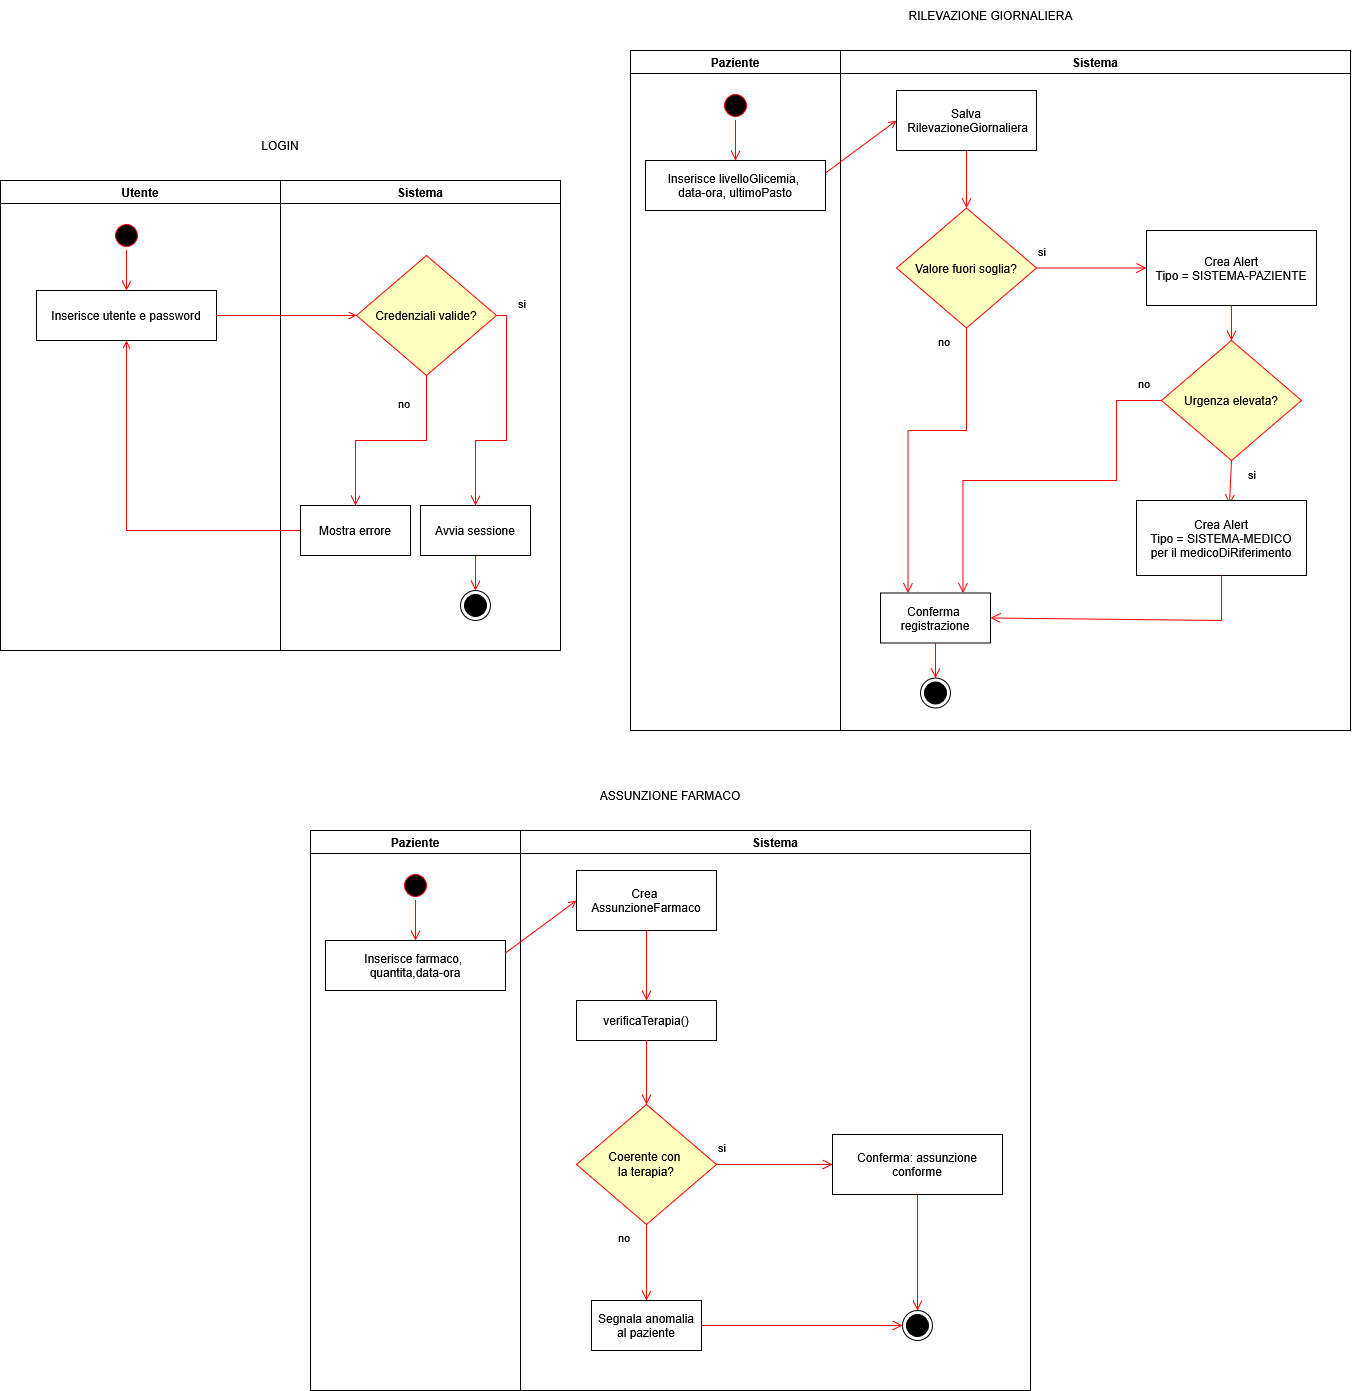
\includegraphics[
		height=0.92\textheight,
		keepaspectratio
		]{Immagini/ActivityDiagram_11.png}
	}
	\caption{Activity Diagram (Parte 1)}
	\label{fig:activity-diagram_1}
\end{figure}


\begin{figure}[H]
	\centering
	\hspace*{-3.5cm}
	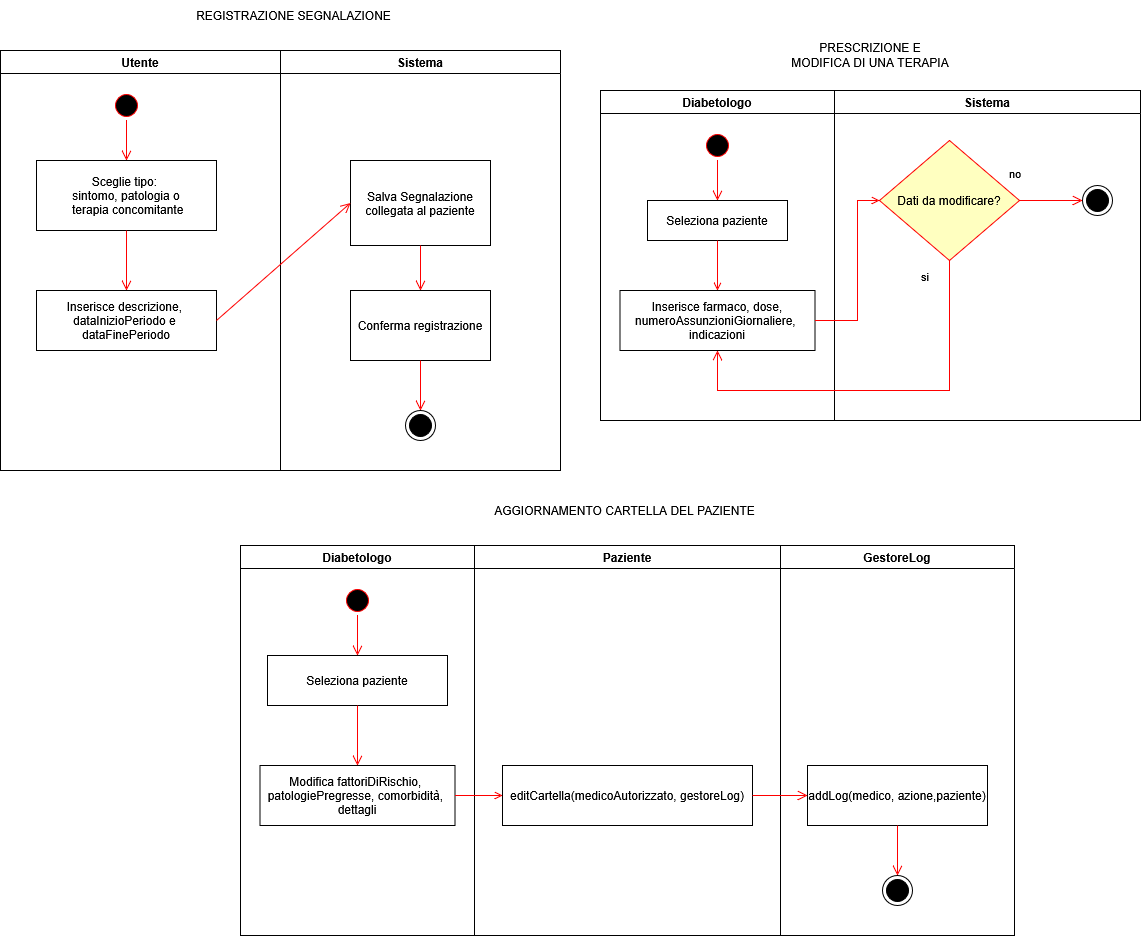
\includegraphics[
	width=0.98\paperwidth,
	height=0.98\textheight,
	keepaspectratio
	]{Immagini/ActivityDiagram_22.png}
	\caption{Activity Diagram (Parte 2)}
	\label{fig:activity-diagram_2}
\end{figure}

 \textcolor{red}{TODO: Idem come il sequence}
	
	\newpage
	\section{Processo di sviluppo}

\subsection{Modelli utilizzati}

Lo sviluppo del progetto è iniziato attraverso la realizzazione di un prototipo contenente la maggior parte delle funzionalità previste. L'obiettivo iniziale era definire e condividere la struttura generale del software, verificando la coerenza tra l'interfaccia grafica, l'esperienza utente, i casi d'uso analizzati e i vincoli imposti dal progetto. Il prototipo ha quindi permesso di verificare fin dalle prime fasi che fossero state considerate tutte le funzionalità necessarie.
Il prototipo disponeva inoltre di una struttura software già organizzata, comprendente le classi del dominio, i controller, le viste FXML, i fogli CSS, le immagini e le altre risorse necessarie. Questa organizzazione ha costituito la base per gli sviluppi successivi, permettendo di concentrarsi sul perfezionamento delle funzionalità senza dover ridefinire la struttura generale dell'applicazione.\\

A partire da questa base è stato adottato un approccio di sviluppo incrementale. Il lavoro è stato suddiviso tra i membri del gruppo, sviluppando progressivamente le funzionalità relative al Responsabile, al Paziente e al Diabetologo e le operazioni che ciascun ruolo può effettuare. Successivamente sono state integrate e perfezionate ulteriori funzionalità trasversali, tra cui la gestione dei messaggi scambiati tra gli utenti e il sistema di registrazione delle modifiche effettuate sui dati dei pazienti.\\
La fase finale è stata dedicata al testing, con l'obiettivo di verificare il corretto funzionamento delle singole componenti e dell'applicazione nel suo complesso.\\

Lo sviluppo del progetto è stato quindi condotto seguendo un approccio di tipo agile, favorito dalle dimensioni ridotte del gruppo, dalla presenza di ruoli definiti e da scadenze frequenti e ravvicinate. Il lavoro è stato svolto principalmente attraverso lo sviluppo e la modifica del codice, con brevi discussioni tra i membri del gruppo prima di apportare le modifiche necessarie. Le funzionalità venivano quindi sviluppate e integrate progressivamente, per poi essere sottoposte a una revisione finale prima dell'approvazione.


\subsection{Stili Architetturali}

Il software segue principalmente un'architettura a strati, nella quale le responsabilità sono suddivise tra interfaccia grafica, logica applicativa e gestione della persistenza.\\
Il Presentation Layer è costituito dalle viste JavaFX e dai relativi controller, che gestiscono l'interazione con l'utente e la visualizzazione dei dati.\\
Il Business Logic Layer comprende le classi del dominio, tra cui User, Paziente, Diabetologo, Terapia, Rilevazione, AssunzioneFarmaco, Segnalazione e le classi responsabili della gestione degli alert e delle regole applicative.\\
Il Data Access Layer è rappresentato dalla classe Database, che centralizza l'accesso ai dati persistenti. I controller e le altre classi che necessitano di recuperare o modificare informazioni persistenti utilizzano il Database come punto di accesso, evitando di gestire direttamente la scrittura sul file. La persistenza viene dunque realizzata tramite serializzazione Java degli oggetti all'interno del file database.data. Nel sistema è inoltre implementato un meccanismo per tracciare le modifiche effettuate sui dati dei pazienti: esse vengono infatti registrate tramite appositi log, consentendo di associare ogni modifica al diabetologo che l'ha effettuata e garantendo così la tracciabilità delle operazioni eseguite.

\subsection{Design Pattern}

Nel progetto è utilizzato il Design Pattern Singleton per la classe Database. Il sistema mantiene infatti una sola istanza condivisa del database, ottenuta tramite il metodo getInstance(). Questo permette di centralizzare l'accesso ai dati e di avere un unico punto di gestione della persistenza durante l'esecuzione dell'applicazione. Un altro utilizzo del Design Pattern Singleton è presente nella classe Session, che mantiene l'utente attualmente autenticato e permette ai diversi controller di accedere alla sessione corrente tramite un'unica istanza condivisa.\\
Il Database espone inoltre metodi specifici per il recupero e la modifica dei dati, ad esempio per ottenere i pazienti associati a un determinato diabetologo, le rilevazioni di un paziente o i messaggi destinati a un medico o a un paziente.\\
Per la gestione della GUI viene utilizzato il pattern Model-View-Controller, attraverso la struttura controller-view di JavaFX. Il pattern prevede la separazione dell'applicazione in tre componenti: il Model, che rappresenta i dati e la logica dell'applicazione, la View, che definisce l'interfaccia grafica, e il Controller, che gestisce le interazioni dell'utente coordinando le operazioni richieste. Nel progetto, il Model è rappresentato dalle classi del dominio, quali, tra le altre, User, Paziente, Diabetologo e Terapia. Le View sono invece definite tramite file FXML e descrivono la struttura e gli elementi grafici delle varie schermate, senza contenere direttamente la logica per la gestione delle operazioni. Infine, i controller, ovvero le apposite classi che gestiscono le View, gestiscono gli eventi originati dall'utente, inizializzando i componenti dell'interfaccia e coordinando le operazioni necessarie al funzionamento. I controller interagiscono inoltre con le classi del dominio e con il database per recuperare, modificare e salvare i dati, aggiornando la View in base al risultato delle operazioni.\\
L'adozione di questa struttura basata sulla divisione delle responsabilità permette di separare la definizione dell'interfaccia dai dati dell'applicazione e dalla gestione degli eventi, rendendo le singole componenti più facilmente comprensibili e manutenibili.

	
	\newpage
	\section{Testing}
Il testing è stato realizzato sulla base dell'approccio White Box. Sono stati sviluppati test relativi sia alle principali classi della business logic e della persistenza dei dati, sia ai controller JavaFX, con l'obiettivo di verificare il corretto comportamento delle varie funzionalità.

\subsection{Unit Test}

Sono stati realizzati test unitari per verificare il comportamento delle principali parti del sistema.\\

Per la classe \texttt{Session} è stato verificato il corretto funzionamento del pattern Singleton, controllando che chiamate multiple a getInstance() restituiscano sempre la stessa istanza. È inoltre stata verificata la corretta gestione dell'utente corrente tramite setCurrentUser(), getCurrentUser() e logout().\\
Per la classe \texttt{Database} sono stati verificati l'inserimento degli utenti senza la creazione di duplicati, la corretta gestione delle associazioni tra pazienti e diabetologi, il recupero delle informazioni relative a un paziente a cui sono stati applicati dei filtri nella ricerca, la gestione dei messaggi e le operazioni di inserimento, modifica ed eliminazione di rilevazioni, assunzioni, segnalazioni e terapie. Riguardo alla gestione delle terapie sono inoltre stati verificati casi quali l'assegnazione a un paziente, il comportamento in caso di assegnazione ripetuta e la modifica di una terapia già assegnata; in particolare, che la modifica di una terapia assegnata a più pazienti comporti la modifica per un paziente soltanto.\\
Per \texttt{GestoreAlert} sono stati verificati casi relativi alla mancata assunzione di farmaci, all'aderenza della terapia per più giorni consecutivi e alla regolarità dei valori glicemici prima e dopo i pasti, considerando soglie che attivino l'invio di alert con diversi livelli di urgenza.\\

Sono inoltre stati realizzati test sui controller dell'applicazione: \\
Sono stati inoltre realizzati test sui controller dell'applicazione. Per \texttt{DiabetologoController} sono state verificate l'inizializzazione della schermata, la visualizzazione dei pazienti associati al medico, la ricerca per nome, cognome e codice fiscale, la gestione della ricerca senza risultati e la corretta apertura delle funzionalità relative ad andamento, terapia e informazioni del paziente.

Per la gestione delle terapie sono stati verificati la visualizzazione e la ricerca delle terapie, l'apertura delle finestre per la creazione e la selezione di terapie esistenti, l'assegnazione e la rimozione delle terapie e il comportamento dei relativi pulsanti.

Per \texttt{MessaggiController} sono stati testati la visualizzazione dei messaggi, la ricerca per mittente, la gestione dei messaggi letti e non letti, la visualizzazione del livello di urgenza e l'aggiornamento delle notifiche.

Per \texttt{PazienteController} sono state verificate le operazioni di inserimento e salvataggio di rilevazioni, assunzioni di farmaci, segnalazioni ed email, compresi i casi di compilazione incompleta dei dati.

Per \texttt{StoricoController} sono state verificate la visualizzazione e la ricerca degli elementi dello storico, le operazioni di modifica con e senza salvataggio e le operazioni di eliminazione.

Infine, per \texttt{ResponsabileController}, \texttt{ModificaCredenzialiController} e \texttt{AggiungiPersonaController} sono state verificate la gestione delle liste di utenti, la ricerca, la modifica dei dati, l'associazione tra pazienti e diabetologi e la creazione di nuovi utenti, compresi i controlli sui dati obbligatori e sugli username già presenti.

\subsection{System Test}
 \textcolor{red}{TODO: Tutto}\\
(Test sull'applicazione completa)\\
Probabili casi da verificare:\\
-Registrazione di una glicemia fuori soglia -$>$ alert $>$ nella dashboard del diabetologo di riferimento\\
-Mancata registrazione di assunzioni farmaco per più di 3 giorni consecutivi -$>$ alert generato al medico\\
-Modifica di una terapia da parte del medico -$>$ le assunzioni successive vengono validate sulla nuova terapia\\
-Login con credenziali errate -$>$ accesso rifiutato\\
-Impossibilità di accedere a dati altrui per chi non ne ha le facoltà\\


	
	
\end{document}
